\scanpage{60}
% block: heading
\uline{Catégorie tannakienne} (sur un corps $k$) \uline{de} \deleted{grou} \uline{lien un groupe diagonalisable} $G=D(\handwritten{\unsure{\Gamma|T}})$ \handwritten{$(\Leftrightarrow\mathcal{M}$} semi-simple, et pour tout objet simple (ou isotypique) $S$ de $\handwritten{\mathcal{M}}$, de rang $d(S)$, $\operatorname{End}(S)$ est de rang $d(S)^{\handwritten{2}}\handwritten{)}$.

% block: classification and first display
Soit $\deleted{M}\handwritten{\mathcal{M}}$ cette c atégorie. Elle est définie à équivalence près (respectant structures et contraintes) par un élément\inserted{\handwritten{$\xi$\begin{tikzpicture}[x=1cm,y=1cm,baseline=0cm]\draw[thin] (-.1,-.4)--(.18,.3);\end{tikzpicture}}} de $H^{\handwritten{2}}(k,G)$. On a d'autre part
\[
H^{\handwritten{2}}(k,G)\handwritten{\simeq}\operatorname{Hom}(\handwritten{\Gamma},\operatorname{Br}(k))\ ,
\]
donc $\handwritten{\mathcal{M}}$ est définie essentiellement par l'homomorphisme \deleted{cano}
\[
\handwritten{\deleted{\unsure{\xi}}u:\ \Gamma\longrightarrow}\operatorname{Br}(k)\ .
\]

% block: grading and characterization
\deleted{Pour tout} La catégorie $\handwritten{\mathcal{M}}$ est graduée de type $\handwritten{\Gamma}$, les objets homogènes de type $\handwritten{\Gamma}$ sont\inserted{\handwritten{les objets\begin{tikzpicture}[x=1cm,y=1cm,baseline=-.1cm]\draw[thin] (0,.06).. controls (.15,-.18) and (-1.1,-.08)..(-1.25,-.3)--(-1.3,-.5);\end{tikzpicture}}} isotypiques, donc pour tout $i\handwritten{\in\Gamma}$, il y a exactement un objet simple, à isomorphisme près, $\unsure{\mathbb{E}|E}_i$, \deleted{de} homogène de degré $i$. (Il semble que ce soit une deuxième caractérisation des catégories tannakiennes de lien $D(\handwritten{\Gamma})$;\inserted{\handwritten{$\Leftrightarrow$ le pr. \unsure{direct|droit|tensl|tensoriel} de deux isotypiques est isotypique\begin{tikzpicture}[x=1cm,y=1cm,baseline=-.1cm]\draw[thin] (0,.06).. controls (.15,-.18) and (-1.1,-.08)..(-1.25,-.3)--(-1.3,-.5);\end{tikzpicture}}}) Le degré de cet élément est égal à l'ordre\inserted{$d(i)$\begin{tikzpicture}[x=1cm,y=1cm,baseline=-.1cm]\draw[thin] (0,.06).. controls (.15,-.18) and (-1.1,-.08)..(-1.25,-.3)--(-1.3,-.5);\end{tikzpicture}} de $u(i)$ dans $\operatorname{Br}(k)$. Donc l'anneau $K(\handwritten{\mathcal{M}})$ est donné par
\[
\begin{aligned}
K(\handwritten{\mathcal{M}})\handwritten{\subset}\underline{Z}\deleted{(}\handwritten{[}\handwritten{\Gamma}\handwritten{]}\ ,\\
\handwritten{\sum}n_i e^i\handwritten{\in}K(\handwritten{\mathcal{M}})\quad\handwritten{\Longleftrightarrow}\quad n_i\handwritten{\equiv}0\ (d(i))\quad\text{pour tout }i\handwritten{\in\Gamma}
\end{aligned}
\]
La base canonique de $K(\handwritten{\mathcal{M}})$ formée par les objets simples étant formée des $d(i)e^i$. Si $M_i$ est l'objet simple de \deleted{poids} degré $i$, alors $\operatorname{End}(M_i)$ est le corps gauche \deleted{de sur} de centre $k$ dont l'invariant daas $\operatorname{Br}(k)$ est $u(i)$.

% block: cancelled paragraph
\deleted{En termes d'un système de générateurs $({}_i)_{i\,\unsure{I|\in I}}$ de $I$, \deleted{et}(d'un système d'objets \deleted{simples}\inserted{isotypiques} \deleted{$\unsure{M|\mathbb{M}}_i$} \deleted{de type} degré $i$)et des}

\figure{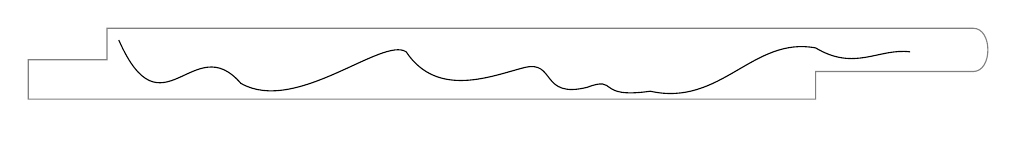
\begin{tikzpicture}[x=1cm,y=1cm]\draw[thin,gray] (0,0)--(0,.4)--(1,.4)--(1,.8)--(12,.8).. controls (12.25,.8) and (12.25,.25)..(12,.25)--(10,.25)--(10,-.1)--(0,-.1)--cycle;\draw (1.15,.65).. controls (1.7,-.6) and (2.1,.8)..(2.7,.1).. controls (3.4,-.3) and (4.5,.7)..(4.8,.5).. controls (5.2,-.1) and (5.9,.2)..(6.3,.3).. controls (6.7,.4) and (6.5,-.1)..(7.1,.05).. controls (7.5,.2) and (7.2,-.1)..(7.9,0).. controls (8.8,-.2) and (9.2,.7)..(10,.55).. controls (10.5,.25) and (10.8,.55)..(11.2,.5);\end{tikzpicture}}

% block: free group case
Si $\Gamma=Z^{(I)}$,\inserted{i.e. $G=G_m^I$,\begin{tikzpicture}[x=1cm,y=1cm,baseline=-.1cm]\draw[thin] (0,.06).. controls (.15,-.18) and (-1.1,-.08)..(-1.25,-.3)--(-1.3,-.5);\end{tikzpicture}} la donnée de $u$\inserted{i.e. de $\handwritten{\xi}$\begin{tikzpicture}[x=1cm,y=1cm,baseline=-.1cm]\draw[thin] (0,.06).. controls (.15,-.18) and (-1.1,-.08)..(-1.25,-.3)--(-1.3,-.5);\end{tikzpicture}} revient à la donnée d'éléments $\handwritten{\xi}_i\handwritten{\in}\operatorname{Br}(k)$. Choisissant pour tout $i$ un objet isotypique non nul de degré $i$, soit $E_i$, et désignant par $A_i=\operatorname{End}(\deleted{\unsure{A|M}}\handwritten{M}_i)$ l'algèbre d'Azymaya associée,\inserted{de classe $\handwritten{\xi}_i$,\begin{tikzpicture}[x=1cm,y=1cm,baseline=-.1cm]\draw[thin] (0,.06).. controls (.15,-.18) and (-1.1,-.08)..(-1.25,-.3)--(-1.3,-.5);\end{tikzpicture}} on réconstitue (à équivalence unique près\deleted{)} respectant tout)
% archive sheet number: 59
